\section{Results}
\label{sec:results}

We report two quantities in this section: the absolute final scores of v1 and v2 with feedback enabled, and the per-epoch training trajectories. The causal-effect ablation appears separately in Section~\ref{sec:ablation}.

\subsection{Final scores}

\begin{table}[H]
\centering
\small
\setlength{\tabcolsep}{6pt}
\begin{tabular}{lccccc}
    \toprule
    \textbf{Model} & $\mathbf{AP}$ & $\mathbf{AP}_S$ & $\mathbf{AP}_M$ & $\mathbf{AP}_L$ & \textbf{Params} \\
    \midrule
    RT-DETR-R50 baseline~\cite{lyu2024rtdetr} & --- & 34.7 & --- & --- & 42.9\,M \\
    Feedback v1 (this work) & 52.01 & 33.91 & 56.28 & 68.83 & 49.1\,M \\
    Feedback v2 (this work) & 52.10 & \textbf{34.25} & 56.33 & 68.82 & 49.1\,M \\
    \bottomrule
\end{tabular}
\caption{Final COCO \textsc{val2017} scores at $640{\times}640$, feedback enabled. v2 yields a $+0.34$ absolute gain on $\mathrm{AP}_S$ over v1. Both models have identical parameter count.}
\label{tab:final}
\end{table}

The absolute gain over v1 is small (Table~\ref{tab:final}). The interesting result is not this comparison --- it is the same-checkpoint ablation in Section~\ref{sec:ablation}, which isolates how much of v2's score is attributable to the feedback computation rather than to the backbone path.

\subsection{Per-epoch trajectories}

Figure~\ref{fig:learning-curves} plots $\mathrm{AP}_S$ over training for v1 and v2. After two chain-restart epochs that look like fresh-start dips (the trainer's optimizer state is reinitialized at SLURM-link boundaries), v2 sits $0.3$--$0.6$ points above v1 at every comparable epoch and crosses v1's eventual final number ($33.91$) at epoch~$8$.

\begin{figure}[H]
    \centering
    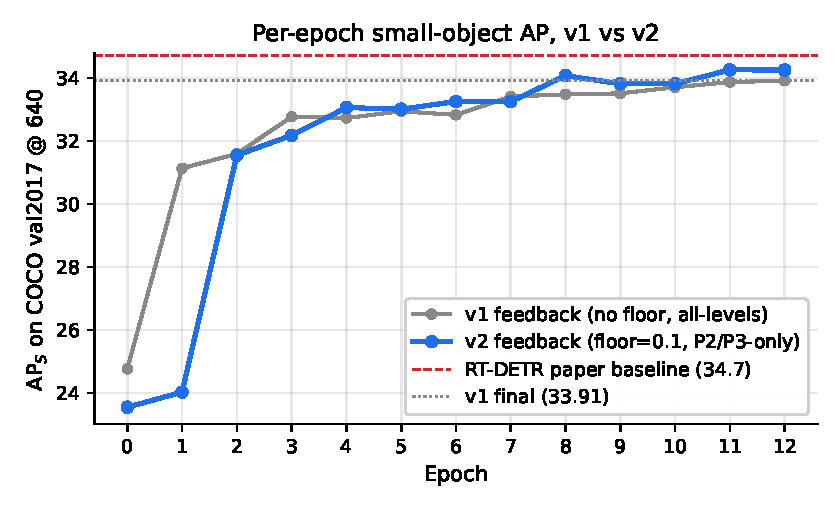
\includegraphics[width=0.78\textwidth]{figures/learning_curves.pdf}
    \caption{Per-epoch $\mathrm{AP}_S$ on COCO \textsc{val2017} at $640{\times}640$. v2 (blue) crosses v1's eventual final $33.91$ at epoch~$8$, four epochs before v1 itself reaches it.}
    \label{fig:learning-curves}
\end{figure}
